\documentclass[11pt,a4paper]{article}
\usepackage[margin=2.6cm]{geometry}
\usepackage{amsmath,amssymb}
\usepackage{graphicx}
\usepackage{booktabs}
\usepackage[font=small,labelfont=bf]{caption}
\usepackage{xcolor}
\usepackage[colorlinks=true,linkcolor=blue!50!black,urlcolor=blue!50!black,citecolor=blue!50!black]{hyperref}
\usepackage{microtype}

\graphicspath{{../figures/}}

% supplementary numbering
\renewcommand{\thesection}{S\arabic{section}}
% widen the TOC number box for two-digit S-numbers
\makeatletter
\renewcommand*\l@section[2]{%
  \ifnum \c@tocdepth >\z@
    \addpenalty\@secpenalty
    \addvspace{1.0em \@plus\p@}%
    \setlength\@tempdima{2.8em}%
    \begingroup
      \parindent \z@ \rightskip \@pnumwidth
      \parfillskip -\@pnumwidth
      \leavevmode \bfseries
      \advance\leftskip\@tempdima
      \hskip -\leftskip
      #1\nobreak\hfil \nobreak\hb@xt@\@pnumwidth{\hss #2}\par
    \endgroup
  \fi}
\makeatother
\renewcommand{\thetable}{S\arabic{table}}
\renewcommand{\thefigure}{S\arabic{figure}}

\newcommand{\lre}{\mathrm{L2RE}}
\newcommand{\eps}{\varepsilon}

\title{\bfseries Supplementary Material:\\
Independent Verification of the 49-Branch Travelling-Wave Catalogue and a
Physics-Informed Neural-Network Benchmark on the Verified Solutions}
\author{Sim2Sci verification study\thanks{Generated from the reproducible
pipeline in \texttt{pinn\_solution\_benchmark/}; every number in this document
is emitted programmatically from the archived raw results
(\texttt{scripts/make\_supplementary.py}).}}
\date{August 25, 2026}

\begin{document}
\maketitle

\noindent This supplement documents, in full, the experiments behind the audit
of the exact-solution catalogue proposed in \emph{paper-5.pdf} for a
fourth-order gain--loss nonlinear Schr\"odinger-type equation, and the
physics-informed neural-network (PINN) benchmark built exclusively on the
solutions that survive independent verification. The study tests whether PINNs
reproduce verified analytical solutions and identifies their success and
failure regimes; it does not claim that PINNs ``work'' in general. Sections
follow the execution order of the pipeline.

\tableofcontents

%=====================================================================
\section{Governing equation, conventions, and the corrected residual split}
\label{sec:eq}

The model is the complex envelope equation
\begin{equation}
\label{eq:pde}
A_z+\frac{i}{2}\left(\beta_2+i g_0T_2^2\right)A_{tt}
+\frac{\beta_3}{6}A_{ttt}
+\frac{i\beta_4}{24}A_{tttt}
+i\left(\gamma+\frac{i\alpha_2}{2}\right)\frac{|A|^2A}{1+\Gamma|A|^2}
+\frac{g_0-\alpha}{2}A=0 ,
\end{equation}
with nine physical coefficients
$(\beta_2,\beta_3,\beta_4,g_0,T_2,\alpha,\alpha_2,\gamma,\Gamma)$. (The source
paper's abstract counts ``eight'' while listing these nine.) Throughout we
abbreviate the only two combinations through which $g_0$, $T_2$ and $\alpha$
enter the algebra,
\begin{equation}
c \equiv g_0T_2^2, \qquad \ell \equiv \tfrac{1}{2}(g_0-\alpha),
\end{equation}
an observation with direct identifiability consequences
(Section~\ref{sec:inverse}).

Writing $A=u+iv$ and
$Q=(u^2+v^2)/\!\left(1+\Gamma(u^2+v^2)\right)$, the real and imaginary
residuals derived symbolically from Eq.~\eqref{eq:pde} are
\begin{align}
F_u&=u_z-\tfrac{c}{2}u_{tt}-\tfrac{\beta_2}{2}v_{tt}
+\tfrac{\beta_3}{6}u_{ttt}-\tfrac{\beta_4}{24}v_{tttt}
-\tfrac{\alpha_2}{2}Qu-\gamma Qv+\ell u,\label{eq:Fu}\\
F_v&=v_z-\tfrac{c}{2}v_{tt}+\tfrac{\beta_2}{2}u_{tt}
+\tfrac{\beta_3}{6}v_{ttt}+\tfrac{\beta_4}{24}u_{tttt}
-\tfrac{\alpha_2}{2}Qv+\gamma Qu+\ell v.\label{eq:Fv}
\end{align}
The identity $F=F_u+iF_v$ is proven in the unit-test suite on random smooth
trial fields and random rational parameter values
(\texttt{tests/test\_symbolic\_math.py}), and the PyTorch automatic-differen\-tiation
implementation is separately tested against the symbolic residual.
The corresponding equations printed in the source paper (its Eqs.~(37)--(38))
fail the same numeric identity check: they attach the $\beta_3$ and $\beta_4$
terms to the wrong field components and leave the complex coefficient
$(\gamma+i\alpha_2/2)$ outside $\mathrm{Re}[\cdot]/\mathrm{Im}[\cdot]$.

%=====================================================================
\section{Audit methodology}
\label{sec:audit}

\paragraph{Ansatz and certificate.}
The paper's ansatz is $A=a\,J_{n,m}(\xi)$, $\xi=\lambda_1z+\lambda_2t$,
$J_{n,m}=\sinh^m\!\xi/\cosh^n\!\xi$, with $a$ real and no carrier phase.
On $\xi>0$ we set $T=\tanh\xi\in(0,1)$ and $W=\operatorname{sech}\xi$. Then
$J_{n,m}=T^mW^{\,n-m}$, the logarithmic derivatives $J^{(k)}/J$ are rational
functions of $T$, and $J^2=T^{2m}(1-T^2)^{\,n-m}$. Substituting the ansatz into
Eq.~\eqref{eq:pde}, dividing by $A$, and clearing only powers of $T$ and
$1-T^2$ --- both nonzero on the open domain --- converts exactness into the
vanishing of all coefficients of a polynomial identity in $T$ (for
half-odd-integer $n-m$, additionally split over the basis $\{1,W\}$, which is
linearly independent over the rational functions of $T$). This certificate is
exhaustive; in particular it does not assume distinct $J$-indices to be
linearly independent, an assumption that underlies the paper's classification
and is false ($J_{2,0}=J_{0,0}-J_{2,2}$, i.e.\
$\operatorname{sech}^2=1-\tanh^2$).

\paragraph{Complete enumeration of closures.}
A bounded recursive factor-splitting solver enumerates every solution family
of each closure system over the unknowns
$(\lambda_1,\lambda_2,a^2,\beta_2,\beta_3,\beta_4,c,\ell,\gamma,\alpha_2,\Gamma)$,
refusing $a=0$ and flagging $\lambda_2=0$ as degenerate. Every terminal family
is then verified through two independent gates:
\begin{enumerate}
\item \textbf{Symbolic gate:} the family's triangular substitutions are
inserted into the certificate with all remaining free parameters kept
symbolic; every coefficient must simplify to exactly zero (this proves the
whole family at once).
\item \textbf{Numeric gate:} exact rational representative parameter sets are
substituted into the \emph{original complex} PDE~\eqref{eq:pde} and the
residual is evaluated at 50-digit precision on a dense $\xi$-grid plus random
$(z,t)$ points, with acceptance thresholds
$\max|F|<10^{-10}$ and $\|F\|_2/\|A\|_2<10^{-10}$ (both configurable; all
accepted families in fact reach $10^{-47}$ or better).
\end{enumerate}
Degenerate candidates are rejected on explicit grounds: $a=0$;
$\lambda_2=0$; identically vanishing governing equation (at most one active
PDE term on the family --- ``vacuous''); denominator singularities inside the
declared domain; residual failure away from any fitting points. Fractional
powers of $\sinh$ are never interpreted silently: the implementation
distinguishes the principal complex power, a signed-real convention, and the
$\xi>0$ restriction, and profiles that are not $C^4$ at $\xi=0$ (the PDE
contains $A_{tttt}$) are either domain-restricted or rejected.

\paragraph{Classification findings.}
Solving the paper's own index-matching requirement
$J_{n+r,m+r}=J_{3n+s,3m+s}$ for both indices simultaneously forces $n=m$
(its Eq.~(28)); the 42 off-diagonal pairs of its $7\times7$ catalogue are
therefore unsupported by its own argument. The audit shows the classification
is also not \emph{necessary}: the only bright branch that genuinely closes,
$(1,0)=\operatorname{sech}$, is off-diagonal.

%=====================================================================
\section{The verified catalogue}
\label{sec:catalog}

Of the 49 proposed pairs, \textbf{9 admit at least one verified nontrivial
solution family; 40 admit only vacuous or $\lambda_2=0$ closures}
(per-pair reasons in \texttt{data/verified\_branches/rejected\_pairs.csv}).
Every surviving family is a \emph{reduced} model: the closure forces several
physical coefficients to zero, and no family supports the full
nine-coefficient equation (no Tier~A solutions under the paper's constant-phase
convention). Table~\ref{tab:catalog} lists the accepted families;
Fig.~\ref{fig:profiles} shows the three benchmark-grade profiles.

\begin{table}[htbp]\centering
\caption{Verified solution families under the paper's constant-phase,
real-amplitude ansatz. ``\#coeffs forced 0'' counts physical coefficients that
the closure sets to zero. Residuals are 50-digit evaluations of
Eq.~\eqref{eq:pde} on dense and random points.}
\label{tab:catalog}
\small
\begin{tabular}{llllrrr}
\toprule
$(n,m)$ & profile & tier & group & \#coeffs forced 0 & $\max|F|$ & rel.\ RMS \\
\midrule
$(0,0)$ & constant & B & main & 1 & $0$ & $0$ \\
$(1,0)$ & bright sech & B & main & 5 & $1.3\times10^{-51}$ & $5.9\times10^{-52}$ \\
$(1,1)$ & dark tanh kink & B & main & 5 & $2.0\times10^{-51}$ & $6.0\times10^{-52}$ \\
$(-1,-1)$ & coth (singular) & B & stress & 5 & $2.1\times10^{-50}$ & $2.4\times10^{-51}$ \\
$(-1,0)$ & cosh (unbounded) & B & stress & 2 & $2.1\times10^{-50}$ & $4.8\times10^{-52}$ \\
$(-1,1)$ & $\tfrac12\sinh(2\xi)$ (unbounded) & B & stress & 2 & $3.8\times10^{-48}$ & $2.5\times10^{-51}$ \\
$(0,-1)$ & csch (singular) & B & stress & 5 & $2.1\times10^{-50}$ & $3.7\times10^{-51}$ \\
$(0,1)$ & sinh (unbounded) & B & stress & 2 & $2.0\times10^{-50}$ & $4.7\times10^{-52}$ \\
$(1,-1)$ & $2\,\mathrm{csch}(2\xi)$ (singular) & B & stress & 5 & $4.3\times10^{-50}$ & $8.4\times10^{-51}$ \\
\bottomrule
\end{tabular}
\end{table}

The closures of the three main-group branches are, explicitly:
\begin{align}
(0,0):&\quad \gamma=0,\quad
\ell=\frac{\alpha_2a^2}{2\left(1+\Gamma a^2\right)}
&&(\text{saturation }\Gamma>0\text{ admitted; }\beta_{2,3,4}\text{ free}),\\
(1,0):&\quad \beta_2=\beta_3=\beta_4=\gamma=\Gamma=0,\;\lambda_1=0,\quad
\alpha_2a^2=2c\lambda_2^2,\;\ \ell=\tfrac{1}{2}c\lambda_2^2,\\
(1,1):&\quad \beta_2=\beta_3=\beta_4=\gamma=\Gamma=0,\;\lambda_1=0,\quad
\alpha_2a^2=-2c\lambda_2^2,\;\ \ell=-c\lambda_2^2 .
\end{align}
Physically, the sech branch is a stationary dissipative bright pulse (net
linear gain balanced by two-photon absorption and spectral filtering) and the
kink is its loss-side mirror (net linear loss balanced by nonlinear gain).
Notably, \emph{no nonconstant branch tolerates saturation} $\Gamma>0$, and the
Kerr coefficient $\gamma$ is forced to zero on every family --- consequences of
the constant-phase convention examined in Section~\ref{sec:extended}.

\begin{figure}[htbp]\centering
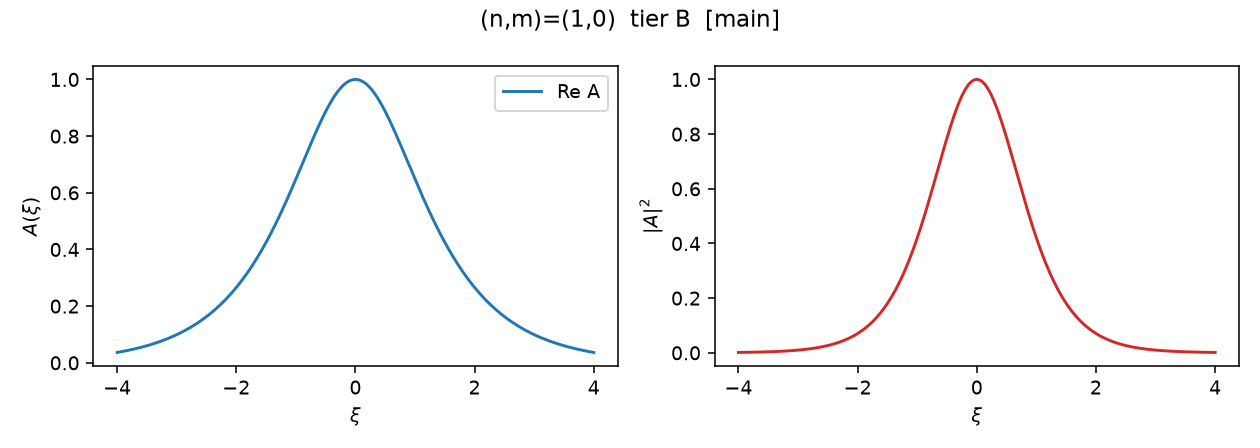
\includegraphics[width=0.49\textwidth]{audit/profile_n1_m0_f0.png}\hfill
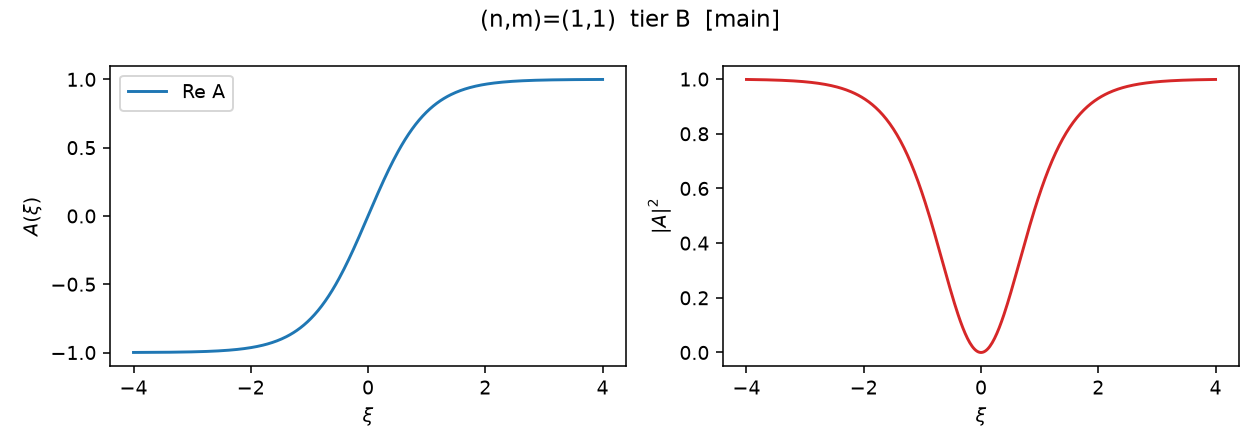
\includegraphics[width=0.49\textwidth]{audit/profile_n1_m1_f0.png}\\[2pt]
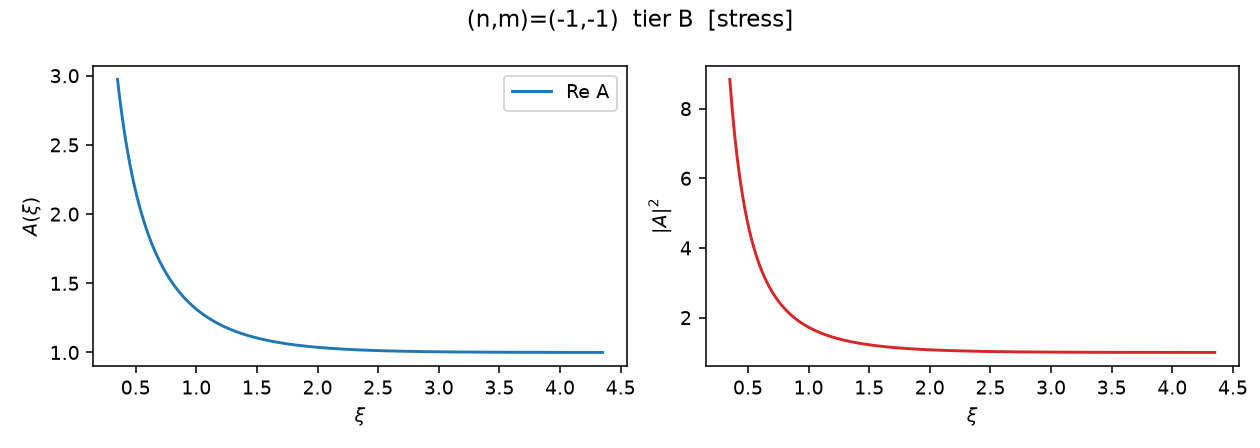
\includegraphics[width=0.49\textwidth]{audit/profile_nneg1_mneg1_f0.png}\hfill
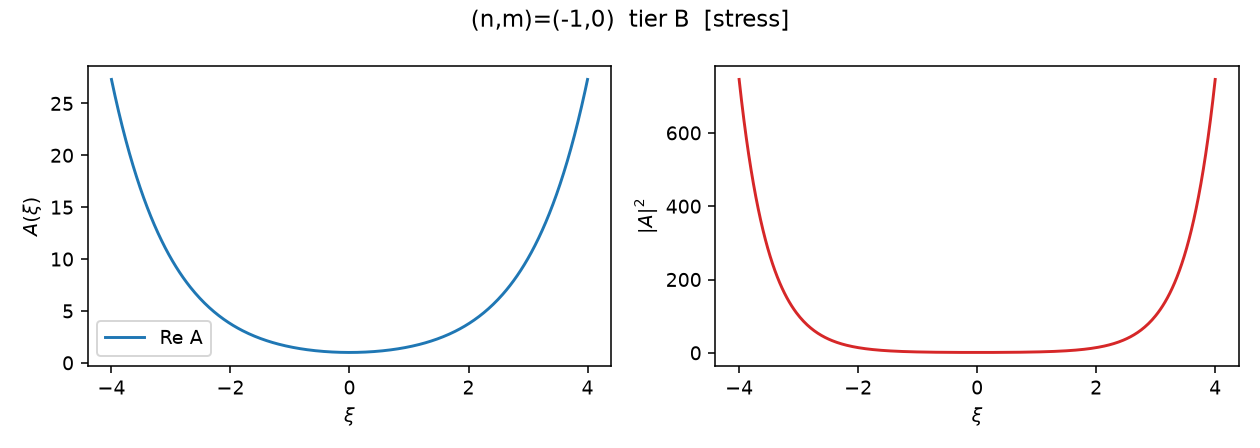
\includegraphics[width=0.49\textwidth]{audit/profile_nneg1_m0_f1.png}
\caption{Verified profiles at their first representative parameter sets.
Top: the two nonconstant main-group branches --- bright sech $(1,0)$ and dark
kink $(1,1)$. Bottom: two stress-group examples --- the singular coth branch
$(-1,-1)$ on its restricted domain $\xi\in[0.35,4.35]$, and the unbounded cosh
branch $(-1,0)$, the latter a solution of the \emph{linear} reduced equation
with third- and fourth-order dispersion active and a genuinely travelling
frame ($\lambda_1=-\beta_3\lambda_2^3/6$).}
\label{fig:profiles}
\end{figure}

%=====================================================================
\section{Optional extended-phase audit}
\label{sec:extended}

As a clearly separated experiment (never a replacement of the paper's
formulation), the full 49-pair audit was repeated for the carrier ansatz
$A=a\,J_{n,m}(\xi)\,e^{i(\kappa z+\omega t)}$. The same two verification gates
apply; all accepted extended families reach residuals
$\approx10^{-51}$. Results: \textbf{17 verified families, all on the same nine
pairs --- none of the 40 rejected pairs is rescued.} The carrier restores
exactly the physics the constant-phase convention destroys:
\begin{itemize}
\item on $(1,0)$, the classic \emph{travelling bright NLS soliton}:
$\gamma=\beta_2\lambda_2^2/a^2$ (focusing), with $\kappa$ the dispersion
relation and $\lambda_1=\beta_2\lambda_2\omega$ the group-velocity shift, in
the conservative reduction $c=\ell=\alpha_2=0$;
\item on $(1,1)$, the \emph{travelling dark soliton}:
$\gamma=-\beta_2\lambda_2^2/a^2$ (defocusing);
\item on $(0,0)$, a \textbf{Tier-A continuous-wave solution} with saturation,
fourth-order dispersion and gain/loss simultaneously active --- the only
full-model solution found anywhere in this study.
\end{itemize}
Conclusion: the catalogue's collapse is caused by the paper's ``$a$ real
without loss of generality'' assumption, not by the equation itself.

%=====================================================================
\section{Independent numerical validation}
\label{sec:numerical}

Each main-group solution was propagated in $z$ by a conventional
method-of-lines solver, entirely independent of the symbolic machinery:
sixth-order central finite differences in $t$ with three ghost nodes per side
filled from the exact analytic boundary data (kinks are never given periodic
boundary conditions), integrated with \textsc{dop853}; for
periodic-compatible profiles (localized or constant) a Fourier pseudospectral
discretization with an ETDRK4 exponential integrator on a $3\times$ padded
window provides a second, structurally different cross-check. The convergence
study covers three spatial resolutions and two integrator tolerances
(Table~\ref{tab:numerical}).

\begin{table}[htbp]\centering
\caption{Convergence study of the independent solver. The finite-difference
scheme exhibits its design order ($\approx6$; the constant branch is at the
rounding floor, where measured ``orders'' are meaningless). The ETDRK4
cross-check on the sech branch is limited to $\sim10^{-6}$ by periodic tail
truncation of the non-periodic profile, as expected.}
\label{tab:numerical}
\small
\begin{tabular}{llrrrrr}
\toprule
branch & scheme & $n_t$ & tol / steps & final L2RE & max err & runtime (s) \\
\midrule
constant $(0,0)$ & fd\_mol & 65 & $1.0\times10^{-8}$ & $9.9\times10^{-12}$ & $1.4\times10^{-11}$ & 0.04 \\
 & fd\_mol & 65 & $1.0\times10^{-10}$ & $1.6\times10^{-13}$ & $2.4\times10^{-13}$ & 0.04 \\
 & fd\_mol & 129 & $1.0\times10^{-8}$ & $8.4\times10^{-12}$ & $1.2\times10^{-11}$ & 0.73 \\
 & fd\_mol & 129 & $1.0\times10^{-10}$ & $2.5\times10^{-13}$ & $4.5\times10^{-13}$ & 0.74 \\
 & fd\_mol & 257 & $1.0\times10^{-8}$ & $5.3\times10^{-11}$ & $7.5\times10^{-11}$ & 13.47 \\
 & fd\_mol & 257 & $1.0\times10^{-10}$ & $1.2\times10^{-12}$ & $1.6\times10^{-12}$ & 13.42 \\
 & ETDRK4 & 256 & 400 steps & $8.6\times10^{-18}$ & $8.6\times10^{-18}$ & 0.06 \\
\multicolumn{7}{l}{\quad\footnotesize observed spatial orders: -0.6, -2.3} \\[2pt]
sech $(1,0)$ & fd\_mol & 65 & $1.0\times10^{-8}$ & $2.3\times10^{-7}$ & $4.4\times10^{-7}$ & 0.01 \\
 & fd\_mol & 65 & $1.0\times10^{-10}$ & $2.3\times10^{-7}$ & $4.4\times10^{-7}$ & 0.02 \\
 & fd\_mol & 129 & $1.0\times10^{-8}$ & $7.6\times10^{-9}$ & $1.2\times10^{-8}$ & 0.05 \\
 & fd\_mol & 129 & $1.0\times10^{-10}$ & $3.7\times10^{-9}$ & $7.2\times10^{-9}$ & 0.05 \\
 & fd\_mol & 257 & $1.0\times10^{-8}$ & $4.6\times10^{-10}$ & $5.0\times10^{-10}$ & 0.20 \\
 & fd\_mol & 257 & $1.0\times10^{-10}$ & $5.8\times10^{-11}$ & $1.2\times10^{-10}$ & 0.21 \\
 & ETDRK4 & 256 & 400 steps & $2.3\times10^{-6}$ & $5.3\times10^{-6}$ & 0.06 \\
\multicolumn{7}{l}{\quad\footnotesize observed spatial orders: 6.0, 6.0} \\[2pt]
kink $(1,1)$ & fd\_mol & 65 & $1.0\times10^{-8}$ & $1.1\times10^{-7}$ & $3.1\times10^{-7}$ & 0.01 \\
 & fd\_mol & 65 & $1.0\times10^{-10}$ & $1.1\times10^{-7}$ & $3.1\times10^{-7}$ & 0.02 \\
 & fd\_mol & 129 & $1.0\times10^{-8}$ & $1.8\times10^{-9}$ & $5.2\times10^{-9}$ & 0.05 \\
 & fd\_mol & 129 & $1.0\times10^{-10}$ & $1.8\times10^{-9}$ & $5.2\times10^{-9}$ & 0.05 \\
 & fd\_mol & 257 & $1.0\times10^{-8}$ & $3.7\times10^{-9}$ & $5.0\times10^{-9}$ & 0.21 \\
 & fd\_mol & 257 & $1.0\times10^{-10}$ & $7.5\times10^{-11}$ & $1.0\times10^{-10}$ & 0.21 \\
\multicolumn{7}{l}{\quad\footnotesize observed spatial orders: 6.0, 4.6} \\[2pt]
\bottomrule
\end{tabular}
\end{table}

Agreement at the $10^{-11}$--$10^{-13}$ level between analytically verified
solutions and an unrelated numerical method confirms the catalogue
independently before any network training.

%=====================================================================
\section{Forward PINN benchmark}
\label{sec:forward}

\paragraph{Setup.}
Networks map $(z,t)\mapsto(\hat u,\hat v)$, $\hat A=\hat u+i\hat v$; all
computations in \texttt{float64}; $\tanh$ activations (smooth through fourth
derivatives); inputs affinely scaled to $[-1,1]$. Training data comprise exact
initial values at $z=0$ and exact Dirichlet values at the two $t$-boundaries
only --- \emph{no interior solution values} --- plus the PDE residual
(Eqs.~\eqref{eq:Fu}--\eqref{eq:Fv}) at Latin-hypercube collocation points.
Errors are evaluated on an independent uniform grid, and residuals on points
never used in training. Three methods: fixed loss weights
($w_{\mathrm{IC}}=w_{\mathrm{BC}}=100$, $w_{\mathrm{PDE}}=1$); gradient-norm
adaptive weighting (Wang et al.\ 2021); residual-adaptive collocation (RAD,
Wu et al.\ 2023). Pilot budget on the available hardware (4-core CPU, no GPU):
$4\times40$ network, 1024 collocation points, 600 Adam + 100 L-BFGS steps
(the recommended GPU configuration --- $6\times64$, $10^4$ points --- ships
unchanged in \texttt{configs/full.yaml}). Matrix: 3~branches $\times$
2~closure-respecting parameter sets $\times$ 3~methods $\times$ 5~seeds
$=90$~runs, \textbf{zero failures}. Success criterion (configurable): complex
$\lre<10^{-2}$ together with a finite independently sampled residual, where
$\lre=\bigl(\sum_j|\hat A_j-A_j|^2/\sum_j|A_j|^2\bigr)^{1/2}$.

\begin{table}[htbp]\centering
\caption{Complete pilot matrix, pooled over the two parameter sets
($n=10$ runs per cell). No selection of favourable seeds: minima and maxima
are shown.}
\label{tab:forward}
\footnotesize
\setlength{\tabcolsep}{4pt}
\begin{tabular}{llrrrrrr}
\toprule
branch & method & $n$ & median & mean $\pm$ std & range & success & resid.\ RMS \\
\midrule
constant $(0,0)$ & fixed weights & 10 & $5.3\times10^{-4}$ & $9.7\times10^{-4}$ $\pm$ $7.8\times10^{-4}$ & $3.4\times10^{-4}$ -- $2.3\times10^{-3}$ & 100\% & $2.2\times10^{-3}$ \\
 & adaptive weights & 10 & $3.8\times10^{-3}$ & $4.1\times10^{-3}$ $\pm$ $3.1\times10^{-3}$ & $2.6\times10^{-4}$ -- $8.6\times10^{-3}$ & 100\% & $6.6\times10^{-3}$ \\
 & adaptive sampling & 10 & $1.3\times10^{-3}$ & $1.6\times10^{-3}$ $\pm$ $1.1\times10^{-3}$ & $2.6\times10^{-4}$ -- $3.4\times10^{-3}$ & 100\% & $3.5\times10^{-3}$ \\
\addlinespace
bright sech $(1,0)$ & fixed weights & 10 & $1.9\times10^{-2}$ & $1.9\times10^{-2}$ $\pm$ $3.3\times10^{-3}$ & $1.4\times10^{-2}$ -- $2.4\times10^{-2}$ & 0\% & $2.6\times10^{-2}$ \\
 & adaptive weights & 10 & $1.3\times10^{-2}$ & $1.5\times10^{-2}$ $\pm$ $8.4\times10^{-3}$ & $4.5\times10^{-3}$ -- $2.9\times10^{-2}$ & 50\% & $1.9\times10^{-2}$ \\
 & adaptive sampling & 10 & $1.6\times10^{-2}$ & $1.7\times10^{-2}$ $\pm$ $3.6\times10^{-3}$ & $1.0\times10^{-2}$ -- $2.4\times10^{-2}$ & 0\% & $2.4\times10^{-2}$ \\
\addlinespace
dark kink $(1,1)$ & fixed weights & 10 & $5.3\times10^{-3}$ & $4.8\times10^{-3}$ $\pm$ $1.1\times10^{-3}$ & $2.9\times10^{-3}$ -- $6.1\times10^{-3}$ & 100\% & $1.8\times10^{-2}$ \\
 & adaptive weights & 10 & $2.4\times10^{-3}$ & $3.1\times10^{-3}$ $\pm$ $1.7\times10^{-3}$ & $1.3\times10^{-3}$ -- $5.9\times10^{-3}$ & 100\% & $9.3\times10^{-3}$ \\
 & adaptive sampling & 10 & $6.0\times10^{-3}$ & $5.5\times10^{-3}$ $\pm$ $1.5\times10^{-3}$ & $3.2\times10^{-3}$ -- $7.4\times10^{-3}$ & 100\% & $1.9\times10^{-2}$ \\
\addlinespace
\bottomrule
\end{tabular}
\end{table}

\begin{figure}[htbp]\centering
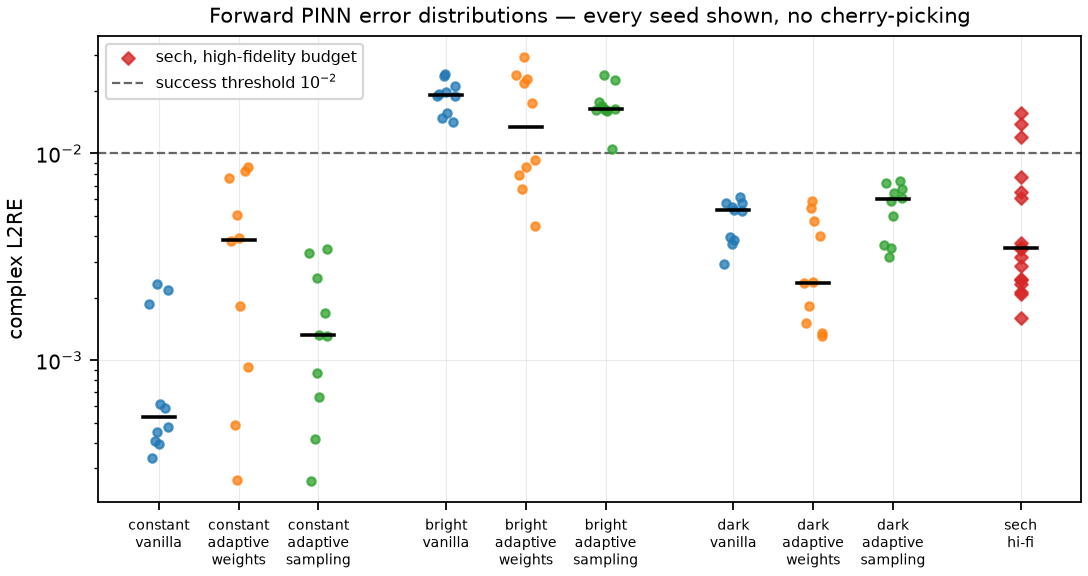
\includegraphics[width=\textwidth]{summary/forward_error_distributions.png}
\caption{Every run of the pilot matrix (dots), medians (bars), and the
high-fidelity sech runs (red diamonds). The constant and kink branches sit
one to two decades below the $10^{-2}$ threshold for every method; the bright
sech branch straddles it at pilot budget.}
\label{fig:dists}
\end{figure}

\begin{figure}[htbp]\centering
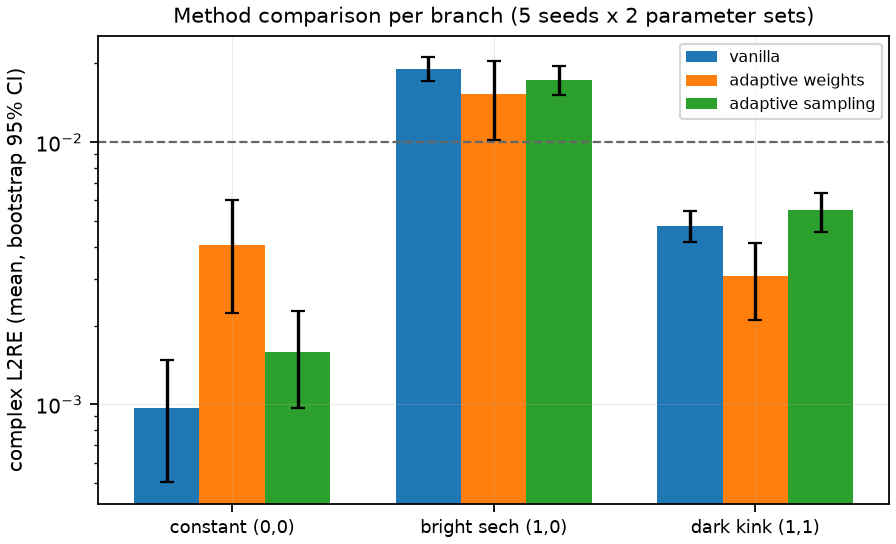
\includegraphics[width=0.55\textwidth]{summary/method_comparison_ci.png}%
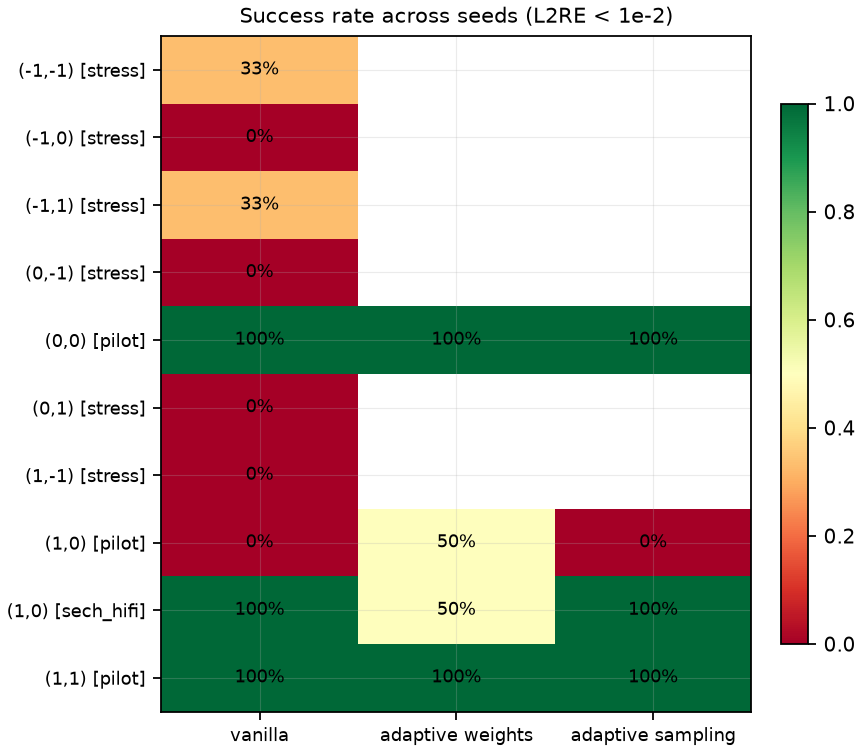
\includegraphics[width=0.44\textwidth]{summary/success_matrix.png}
\caption{Left: per-branch method comparison with bootstrap 95\% confidence
intervals. Right: success rates across seeds for all forward experiments,
including the stress group and the high-fidelity sech rerun.}
\label{fig:methods}
\end{figure}

\begin{figure}[htbp]\centering
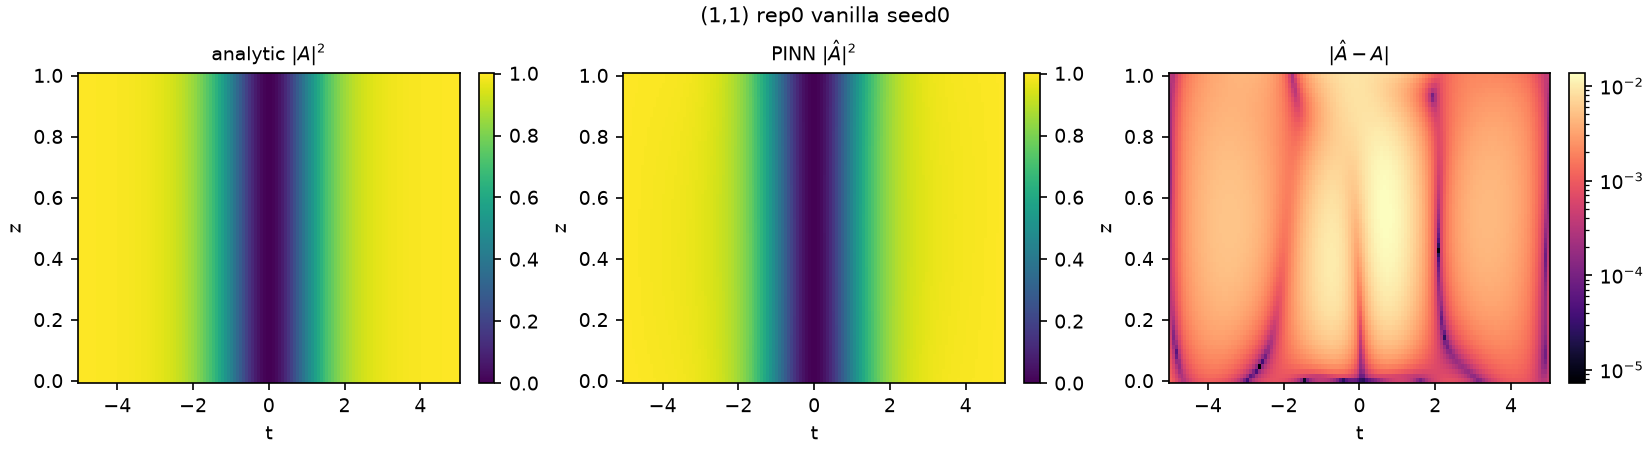
\includegraphics[width=\textwidth]{forward_pilot/field_forward_pilot__n1_m1_f0__rep0__vanilla__seed0.png}\\[2pt]
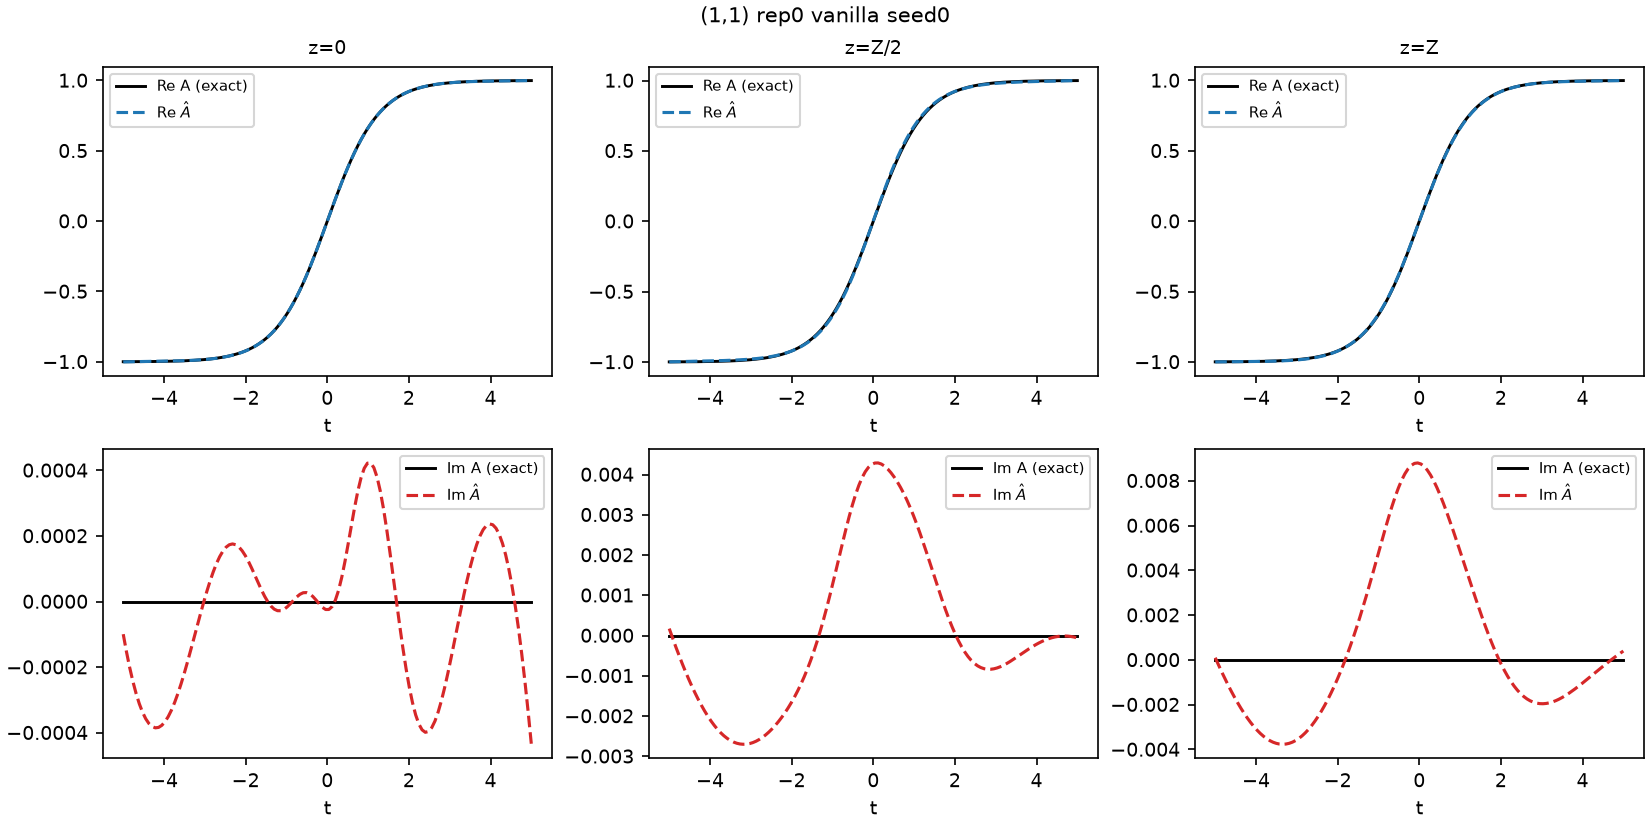
\includegraphics[width=\textwidth]{forward_pilot/sections_forward_pilot__n1_m1_f0__rep0__vanilla__seed0.png}
\caption{Representative reconstruction (dark kink, fixed weights, median
seed). Top: analytic intensity $|A|^2$, PINN intensity, and pointwise complex
error. Bottom: real and imaginary components at $z=0$, $Z/2$, $Z$; the network
must also learn that $\mathrm{Im}\,A\equiv0$.}
\label{fig:field}
\end{figure}

\begin{figure}[htbp]\centering
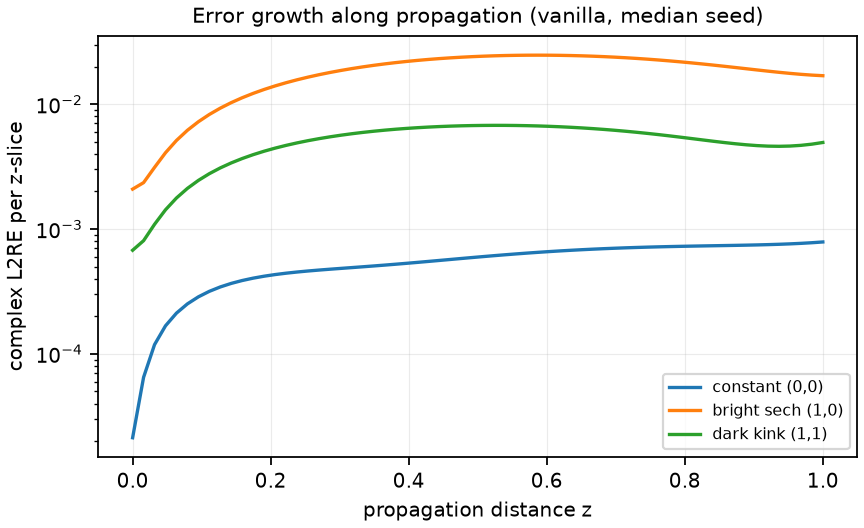
\includegraphics[width=0.62\textwidth]{summary/error_vs_z_branches.png}
\caption{Per-slice error along the propagation direction (fixed weights,
median seeds). Errors are anchored by the exact data at $z=0$ and grow into
the interior, where the residual term alone carries the solution.}
\label{fig:evz}
\end{figure}

\paragraph{Findings.}
(i)~Difficulty is ordered exactly as predicted by the catalogue's
shape features: constant $<$ kink $<$ sech, tracking the maxima of $|A_{tt}|$
and, dominantly, $|A_{tttt}|$ --- the operative feature given the equation's
fourth-derivative term (Fig.~\ref{fig:difficulty}).
(ii)~Adaptive loss weighting is the only method to lift the sech branch to
$50\%$ success at pilot budget, while \emph{degrading} the easiest branch
(it deprioritizes already-converged data terms); adaptive collocation helps
the constant branch and is neutral elsewhere.

\begin{figure}[htbp]\centering
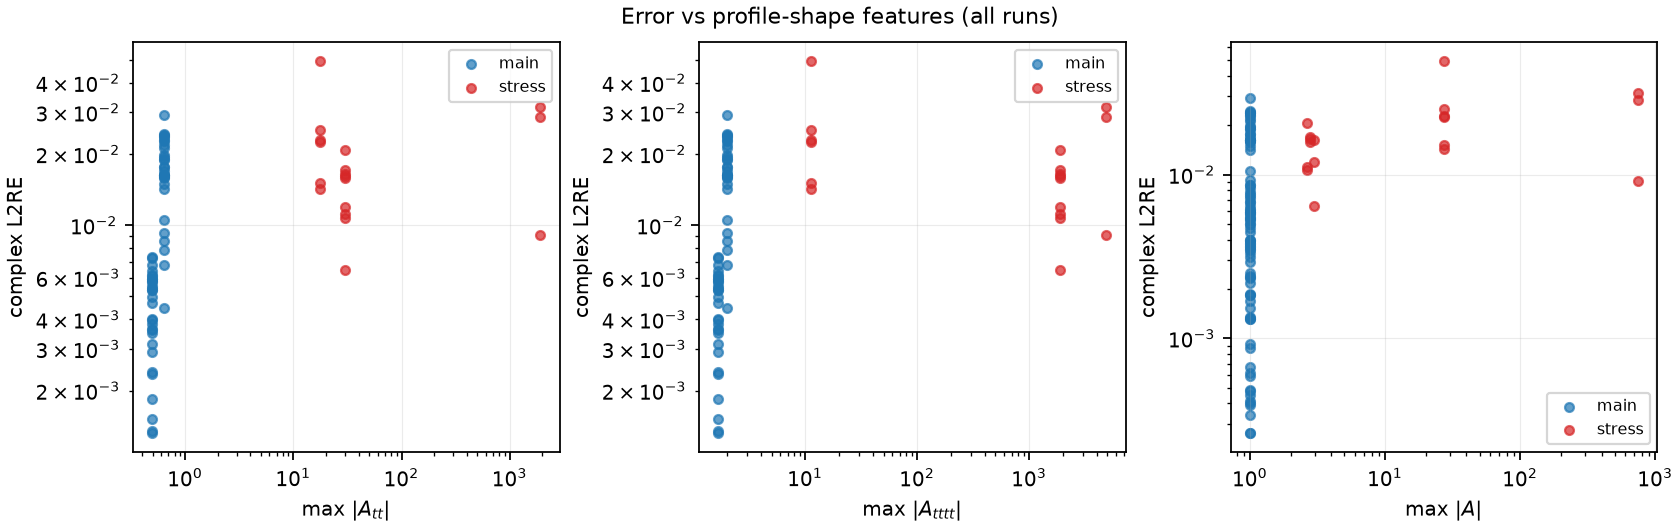
\includegraphics[width=\textwidth]{summary/difficulty_features.png}
\caption{Error against profile-shape features for all forward runs (main and
stress groups). The correlation with the fourth-derivative magnitude is the
strongest of the three.}
\label{fig:difficulty}
\end{figure}

\subsection{High-fidelity rerun of the failing branch}
\label{sec:hifi}

To decide whether the sech failure is fundamental or budget-limited, the
branch was retrained at $2.5\times$ the optimization steps and $2\times$ the
collocation points ($4\times48$ network; 18 runs). Median $\lre$ falls from
$1.6\times10^{-2}$ to $3.5\times10^{-3}$ with \textbf{83\% overall success}
(Table~\ref{tab:hifi}): the pilot-budget failure is largely a \emph{budget
artifact}. The rerun also reverses the method ranking --- fixed weights and
adaptive sampling reach $100\%$ success while adaptive weighting drops to
$50\%$: \textbf{method rankings are budget-dependent}, a caution against
comparing PINN variants at a single training budget.

\begin{table}[htbp]\centering
\caption{High-fidelity sech runs (2500 Adam + 300 L-BFGS steps, 2048 points).}
\label{tab:hifi}
\small
\begin{tabular}{lrrrr}
\toprule
method & $n$ & median L2RE & range & success \\
\midrule
fixed weights & 6 & $3.5\times10^{-3}$ & $2.1\times10^{-3}$ -- $6.5\times10^{-3}$ & 100\% \\
adaptive weights & 6 & $7.8\times10^{-3}$ & $1.6\times10^{-3}$ -- $1.6\times10^{-2}$ & 50\% \\
adaptive sampling & 6 & $2.7\times10^{-3}$ & $2.1\times10^{-3}$ -- $7.7\times10^{-3}$ & 100\% \\
\midrule
all methods & 18 & $3.5\times10^{-3}$ & $1.6\times10^{-3}$ -- $1.6\times10^{-2}$ & 83\% \\
\bottomrule
\end{tabular}
\end{table}

\subsection{Stress group}
\label{sec:stress}

The six stress branches --- singular profiles on domains bounded away from
$\xi=0$, and unbounded cosh/sinh-type solutions of the linear reduced equation
with $\beta_3,\beta_4$ active and travelling frames --- were trained for the
first time at pilot budget (18 runs, fixed weights,
Table~\ref{tab:stress}). All six sit at or above the success threshold
(medians $1.1$--$2.9\times10^{-2}$, success $0$--$33\%$): near-singular
gradients, field amplitudes up to $\sim27$, and active high-order dispersion
each cost one to two decades relative to the main group. These branches
delimit the failure regime of the benchmark and are reported without
selection.

\begin{table}[htbp]\centering
\caption{Stress-group results (fixed weights, 3 seeds per branch).}
\label{tab:stress}
\small
\begin{tabular}{llrrrr}
\toprule
$(n,m)$ & profile & $n$ & median L2RE & range & success \\
\midrule
$(-1,-1)$ & coth kink (singular) & 3 & $1.2\times10^{-2}$ & $6.4\times10^{-3}$ -- $1.6\times10^{-2}$ & 33\% \\
$(-1,0)$ & cosh (unbounded, $\beta_3,\beta_4$ active) & 3 & $2.5\times10^{-2}$ & $2.3\times10^{-2}$ -- $4.9\times10^{-2}$ & 0\% \\
$(-1,1)$ & $\tfrac12\sinh(2\xi)$ (unbounded, travelling) & 3 & $2.9\times10^{-2}$ & $9.1\times10^{-3}$ -- $3.2\times10^{-2}$ & 33\% \\
$(0,-1)$ & csch pulse (singular) & 3 & $1.6\times10^{-2}$ & $1.6\times10^{-2}$ -- $1.7\times10^{-2}$ & 0\% \\
$(0,1)$ & sinh (unbounded, travelling) & 3 & $1.5\times10^{-2}$ & $1.4\times10^{-2}$ -- $2.3\times10^{-2}$ & 0\% \\
$(1,-1)$ & $2\,\mathrm{csch}(2\xi)$ (singular) & 3 & $1.1\times10^{-2}$ & $1.1\times10^{-2}$ -- $2.1\times10^{-2}$ & 0\% \\
\bottomrule
\end{tabular}
\end{table}

%=====================================================================
\section{Inverse parameter discovery}
\label{sec:inverse}

\paragraph{Identifiability first.}
Because $g_0$, $T_2$, $\alpha$ enter Eq.~\eqref{eq:pde} only through $c$ and
$\ell$, they cannot be separately recovered from any single field. The
sensitivity Jacobian $\partial F/\partial\theta$ evaluated on the exact
solutions confirms this numerically: rank $2$ of $3$ in
$(g_0,T_2,\alpha)$ with an explicit null direction, and rank $7$ of $8$ with
condition number $\sim10^{11}$ in the reduced coordinates
(Table~\ref{tab:ident}). All recovery is therefore performed in
$\theta=(\beta_2,\beta_3,\beta_4,c,\ell,\gamma,\alpha_2,\Gamma)$, with
positive parameters ($c,\Gamma$) in softplus parameterization and all
parameters scaled to $O(1)$.

\begin{table}[htbp]\centering
\caption{Sensitivity analysis on the exact solutions (400 random points).
The near-zero third singular value in $(g_0,T_2,\alpha)$ and its null
direction prove joint non-identifiability; recovery targets $c$ and $\ell$
instead.}
\label{tab:ident}
\small
\begin{tabular}{lrrrl}
\toprule
branch & reduced rank & cond.\ number & $(g_0,T_2,\alpha)$ rank & null direction \\
\midrule
kink $(1,1)$ & 7/8 & $7.6\times10^{10}$ & 2/3 & $(-0.686, 0.243, -0.686)$ \\
sech $(1,0)$ & 7/8 & $1.1\times10^{11}$ & 2/3 & $(-0.686, 0.243, -0.686)$ \\
\bottomrule
\end{tabular}
\end{table}

\paragraph{Staged recovery.}
Network and parameters are trained jointly from sparse noisy interior
observations plus the residual (1200 Adam steps; initial parameter guesses
offset by $\pm50\%$; five seeds configured, three executed per cell on this
hardware; both an easy branch --- the kink --- and the hardest --- the sech).
Noise is Gaussian with standard deviation quoted relative to the field's
standard deviation. Results: Table~\ref{tab:invnoise} and
Fig.~\ref{fig:inverse}.

\begin{table}[htbp]\centering
\caption{Median recovery error at 5\% observation density, by stage and noise
level (both branches pooled; median over seeds). For parameters whose true
value is $0$ the entry is the \emph{absolute} error --- these rows measure the
ability to \emph{discover} that a term is absent.}
\label{tab:invnoise}
\small
\begin{tabular}{llrrrr}
\toprule
stage & parameter & 0\% noise & 1\% noise & 5\% noise & runs \\
\midrule
gainloss & $c=g_0T_2^2$ & $1.8\times10^{-2}$ & $3.0\times10^{-2}$ & $6.4\times10^{-2}$ & 6 \\
 & $\ell=(g_0-\alpha)/2$ & $3.3\times10^{-3}$ & $7.3\times10^{-3}$ & $2.2\times10^{-2}$ & 6 \\
\addlinespace
nonlinear & $\gamma$ (true 0) & $1.5\times10^{-3}$ & $7.3\times10^{-4}$ & $2.5\times10^{-3}$ & 6 \\
 & $\Gamma$ (true 0) & $2.3\times10^{-2}$ & $2.4\times10^{-2}$ & $3.0\times10^{-2}$ & 6 \\
 & $\alpha_2$ & $1.5\times10^{-2}$ & $1.2\times10^{-2}$ & $2.4\times10^{-2}$ & 6 \\
\addlinespace
dispersion & $\beta_2$ (true 0) & $9.1\times10^{-3}$ & $6.9\times10^{-3}$ & $1.8\times10^{-2}$ & 6 \\
 & $\beta_3$ (true 0) & $2.6\times10^{-2}$ & $2.1\times10^{-2}$ & $7.2\times10^{-2}$ & 6 \\
 & $\beta_4$ (true 0) & $4.3\times10^{-2}$ & $6.6\times10^{-2}$ & $7.7\times10^{-2}$ & 6 \\
\addlinespace
\bottomrule
\end{tabular}
\end{table}

\begin{figure}[htbp]\centering
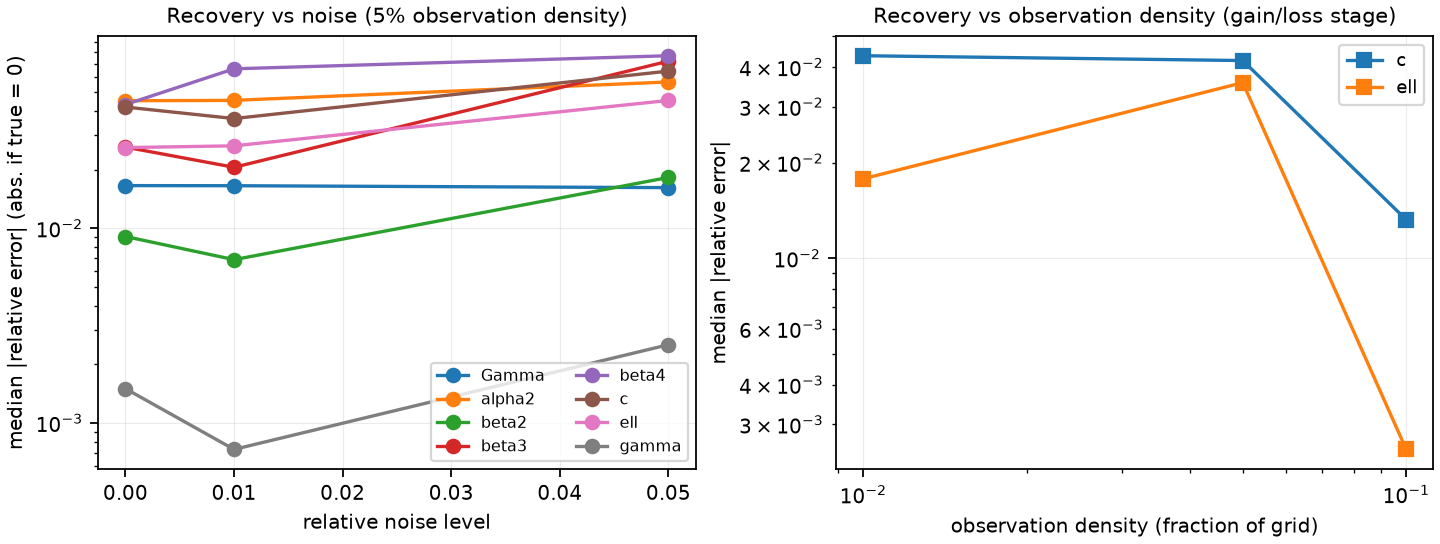
\includegraphics[width=\textwidth]{summary/inverse_recovery.png}
\caption{Left: median recovery error against noise at 5\% density. Right:
recovery of the gain/loss combinations against observation density (1\%, 5\%,
10\%) --- a clean monotone improvement.}
\label{fig:inverse}
\end{figure}

\begin{table}[htbp]\centering
\caption{Observation-density sweep for the gain/loss stage (noise levels
pooled; median over seeds and branches).}
\label{tab:invdens}
\small
\begin{tabular}{lrrr}
\toprule
parameter & 1\% density & 5\% density & 10\% density \\
\midrule
$c=g_0T_2^2$ & $4.3\times10^{-2}$ & $3.0\times10^{-2}$ & $1.3\times10^{-2}$ \\
$\ell=(g_0-\alpha)/2$ & $1.8\times10^{-2}$ & $7.6\times10^{-3}$ & $2.5\times10^{-3}$ \\
\bottomrule
\end{tabular}
\end{table}

\begin{table}[htbp]\centering
\caption{Staged versus joint recovery. Joint four-parameter recovery degrades
by roughly an order of magnitude for the genuinely nonzero parameters,
consistent with the $\sim10^{11}$ conditioning of the sensitivity matrix.}
\label{tab:invjoint}
\small
\begin{tabular}{lrrr}
\toprule
parameter & staged (median) & joint 4-param (median) & joint runs \\
\midrule
$c=g_0T_2^2$ & $3.0\times10^{-2}$ & $1.2\times10^{-1}$ & 18 \\
$\ell=(g_0-\alpha)/2$ & $7.6\times10^{-3}$ & $1.6\times10^{-1}$ & 18 \\
$\alpha_2$ & $1.7\times10^{-2}$ & $1.5\times10^{-1}$ & 18 \\
$\Gamma$ (true 0) & $2.3\times10^{-2}$ & $1.5\times10^{-2}$ & 18 \\
\bottomrule
\end{tabular}
\end{table}

\paragraph{Findings.}
(i)~The identifiable gain/loss combinations are the best-recovered quantities
($\ell$ to $0.3$--$2\%$, $c$ to $1$--$7\%$ across $0$--$5\%$ noise), degrading
gracefully with noise and improving monotonically with density
(Table~\ref{tab:invdens}).
(ii)~The nonlinear stage recovers $\alpha_2$ to $1$--$3\%$ and correctly
discovers $\gamma\approx0$ and $\Gamma\approx0$.
(iii)~The dispersion stage is the weakest: the $\beta$'s (true value $0$ on
these branches) are pinned only to median absolute error
$3.3\times10^{-2}$ --- high-order derivative terms have weak sensitivity on
smooth solutions.
(iv)~Joint recovery is much harder than staged recovery
(Table~\ref{tab:invjoint}).
(v)~A structural consequence of the audit: on the surviving branches most
coefficients are \emph{forced to zero}, so the paper's proposed
nine-parameter recovery benchmark largely reduces to discovering zeros.

%=====================================================================
\section{Physical ablations}
\label{sec:ablations}

Matched pairs change exactly one closure-consistent quantity on the constant
branch --- the only branch whose closure admits them
(Table~\ref{tab:ablations}). Saturation ($\Gamma:0\to1$) and fourth-order
dispersion in the operator ($\beta_4:0\to0.4$) each make the forward problem
mildly harder ($\times1.2$--$1.4$ in mean $\lre$). The remaining requested
ablations are \emph{impossible by closure}, which is itself a reportable
finding: no verified branch admits a conservative version
($\ell=\alpha_2=0$ collapses every family), and $\Gamma>0$ or $\beta_4\neq0$
are closure-forbidden off the constant branch --- the verified solution set is
intrinsically dissipative. Fixed-versus-adaptive weighting and
uniform-versus-adaptive sampling are covered by the factorial matrix of
Section~\ref{sec:forward}.

\begin{table}[htbp]\centering
\caption{Matched ablations (3 seeds per arm, fixed weights, 800 Adam + 150
L-BFGS steps).}
\label{tab:ablations}
\small
\begin{tabular}{lrr}
\toprule
arm (constant branch, one closure-consistent change) & mean L2RE $\pm$ std & $n$ \\
\midrule
saturation off ($\Gamma=0$) & $6.1\times10^{-4}$ $\pm$ $2.1\times10^{-4}$ & 3 \\
saturation on ($\Gamma=1$) & $8.8\times10^{-4}$ $\pm$ $3.0\times10^{-4}$ & 3 \\
$\beta_4=0$ & $9.2\times10^{-4}$ $\pm$ $3.5\times10^{-4}$ & 3 \\
$\beta_4=0.4$ & $1.1\times10^{-3}$ $\pm$ $6.7\times10^{-4}$ & 3 \\
\bottomrule
\end{tabular}
\end{table}

%=====================================================================
\section{Parameter-conditioned cross-branch PINN}
\label{sec:conditioned}

A network taking only $(z,t)$ cannot represent multiple solutions at the same
coordinates, so generalization experiments use
$\hat A_\theta(z,t;\eta)$ with
$\eta=(n,m,a,\lambda_1,\lambda_2,\beta_2,\beta_3,\beta_4,c,\ell,\gamma,
\alpha_2,\Gamma)$ scaled over the task pool. Training tasks are the catalogue
representatives of the training branches; evaluation tasks at new parameters
are generated \emph{only} by re-solving the exact closure constraints at new
free-parameter values, never by free perturbation. Train/held-out branch lists
are explicit in \texttt{configs/generalization\_pilot.yaml}; in
leave-one-branch-out (LOBO) runs the held-out branch contributes nothing to
training, and fine-tuning uses only the stated fraction of held-out interior
data (two seeds).

\begin{table}[htbp]\centering
\caption{Conditioned-PINN transfer, mean $\lre$ over seeds and the two
held-out parameter sets. ``Scratch, same budget'' trains a fresh
single-branch network for exactly the fine-tuning step budget.}
\label{tab:gen}
\small
\begin{tabular}{lrrrr}
\toprule
held-out branch & zero-shot & fine-tune 1\% & fine-tune 5\% & scratch, same budget \\
\midrule
constant $(0,0)$ & $7.1\times10^{-1}$ & $8.3\times10^{-3}$ & $6.2\times10^{-3}$ & $1.1\times10^{-2}$ \\
sech $(1,0)$ & $1.3\times10^{0}$ & $6.7\times10^{-2}$ & $4.8\times10^{-2}$ & $9.9\times10^{-2}$ \\
kink $(1,1)$ & $1.1\times10^{0}$ & $6.0\times10^{-2}$ & $2.5\times10^{-2}$ & $5.8\times10^{-2}$ \\
\multicolumn{5}{l}{interpolation (all branches): mean L2RE $1.3\times10^{-1}$} \\
\multicolumn{5}{l}{extrapolation (all branches): mean L2RE $6.7\times10^{-1}$} \\
\bottomrule
\end{tabular}
\end{table}

\begin{figure}[htbp]\centering
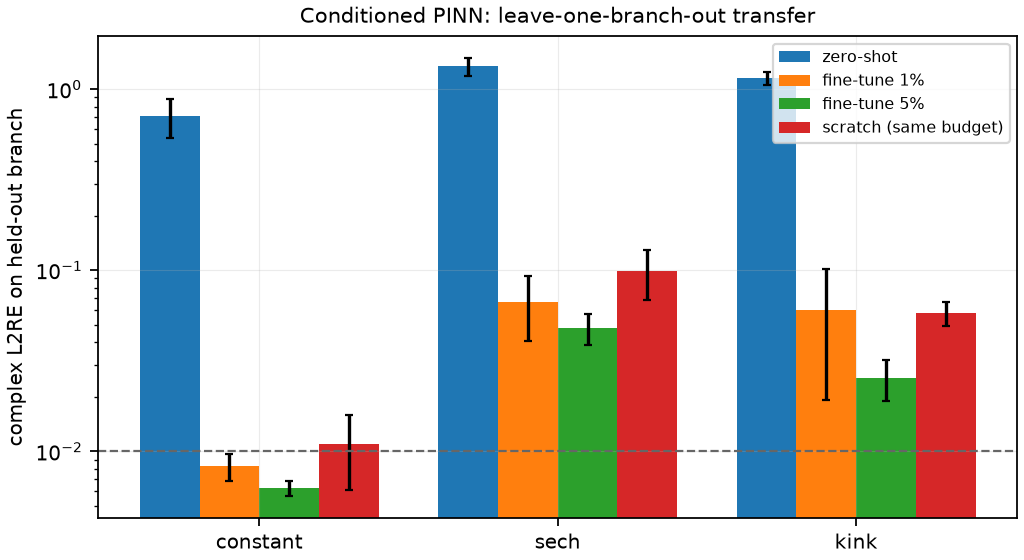
\includegraphics[width=0.49\textwidth]{summary/generalization_lobo.png}\hfill
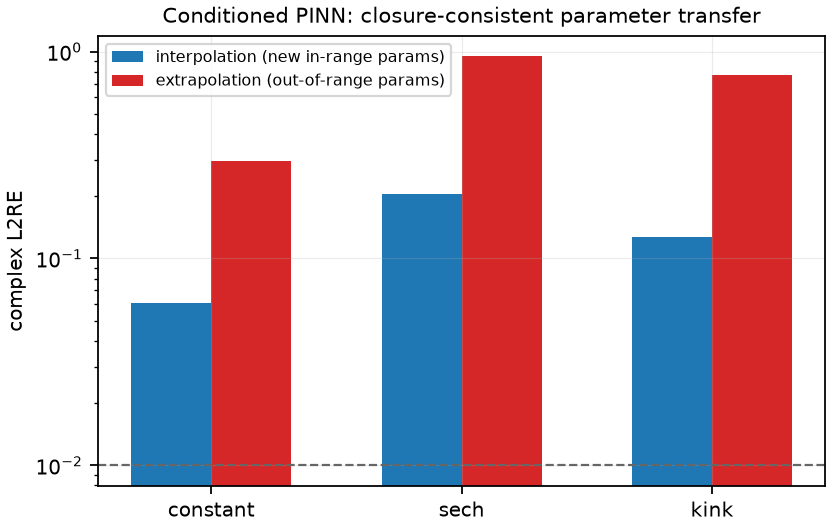
\includegraphics[width=0.49\textwidth]{summary/generalization_interp_extrap.png}
\caption{Left: LOBO transfer --- zero-shot fails ($\lre\approx1$); 1\% of
held-out data recovers scratch-level or better accuracy at matched compute.
Right: transfer to new closure-consistent parameters --- interpolation
partially succeeds, extrapolation fails.}
\label{fig:gen}
\end{figure}

\paragraph{Findings.}
Zero-shot transfer to an unseen branch fails completely
($\lre\approx0.7$--$1.3$): the conditioning vector does not let the network
infer a qualitatively different profile shape it has never seen --- an
expected but now quantified negative result. Interpolation to unseen in-range
parameters of \emph{seen} branches partially succeeds
(mean $1.3\times10^{-1}$); extrapolation fails (mean $6.7\times10^{-1}$).
Fine-tuning with 1\% of held-out data restores accuracy comparable to --- on
two of three branches better than --- a from-scratch network at the same step
budget, so the shared representation carries some reusable structure.

%=====================================================================
\section{Reproducibility, compute, and honest scope}
\label{sec:repro}

\paragraph{Environment.} Linux, 4-core CPU, no GPU; Python 3.12; PyTorch
(CPU, \texttt{float64}), SymPy/mpmath for the audit (50-digit arithmetic);
all package versions logged per experiment in
\texttt{results/*/environment.json}. Seeds are fixed and recorded; per-run raw
results are archived before aggregation; checkpointing allows every experiment
to resume, and completed jobs are skipped unless \texttt{--force} is passed.
The complete unit-test suite (42 tests: symbolic derivatives, residual-split
identity, autodiff-versus-symbolic derivatives, fourth-derivative accuracy,
fractional-power conventions, singularity detection, closure verification,
degenerate rejection, metrics, leakage, deterministic seeding,
checkpoint/resume, end-to-end smoke) passes before and after all experiments.

\paragraph{Compute scale.} Roughly 230 training runs are archived: 90 pilot,
18 high-fidelity sech, 18 stress, 108 inverse, plus conditioned-PINN
trainings and matched ablations. Network and collocation sizes are the
documented CPU scaling of the recommended settings; the single configuration
not executed end-to-end on this machine is the GPU-scale
\texttt{configs/full.yaml} ($6\times64$, $10^4$ collocation points, 5000+500
steps), which is expected to move absolute errors down without changing the
qualitative orderings established here --- the high-fidelity sech rerun
(Section~\ref{sec:hifi}) is direct evidence for that trend. Inverse cells ran
3 of the 5 configured seeds.

\paragraph{Commands.}
\begin{verbatim}
python scripts/run_audit.py --config configs/audit.yaml   # +--extended-phase
python -m pytest tests/ -q
python scripts/run_numerical.py
python scripts/run_forward.py --config configs/pilot.yaml
python scripts/run_forward.py --config configs/sech_highfidelity.yaml
python scripts/run_forward.py --config configs/stress.yaml
python scripts/run_inverse.py  --config configs/inverse_pilot.yaml
python scripts/run_ablations.py
python scripts/run_generalization.py --config configs/generalization_pilot.yaml
python scripts/run_full_benchmark.py --mode smoke|pilot|full   # whole pipeline
\end{verbatim}

\paragraph{Provenance of claims.} Mathematically proven: every family in
\texttt{branch\_catalog.json} (symbolic zero + 50-digit residuals).
Unsupported: the 40 rejected pairs, with per-pair reasons. PINN successes and
failures: per-run \texttt{result.json} files under \texttt{results/}; raw
errors are always retained and no seed is excluded anywhere in this document.

\end{document}
